\section{Readout}\label{ssec:readout}
In \cref{ssec:SPADs} two circuitry components where mentioned that are required for each SPAD: a ROIC and a TDC. While the decision on whether or not to push out the ROIC has not yet been made, \cref{ssec:SPAD_layout} concluded that it is necessary to push out the TDC. One other important aspect of the TDC is that it must meet the designed resolution of $50\,ps$. The proposed TDC design uses a Phase Locked Loop (PLL) to generate signals that the TDC can use to time stamp an incoming pulse. The PLL, for which a schematic is shown in \cref{tkz:PLL}, locks onto an input in such a way, that both signals entering the phase detector are equal. By using a divider by $X$ block, one can generate a signal with a frequency that is equal to $x$ times the clock frequency. The voltage controlled oscillator is capable of generating 4 signals with 4 different phases to increase the resolution further. \Cref{tkz:TDC_line_PLL} shows a line of TDCs connected to the PLL.
		
\begin{figure}[H]
    \centering

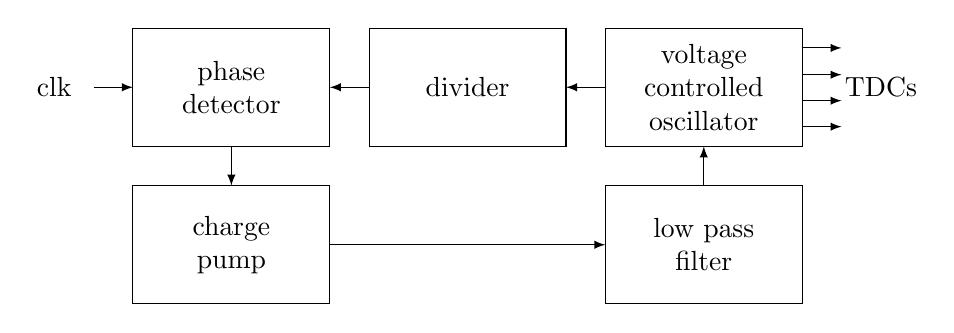
\begin{tikzpicture}

\draw  (-2,1.75) rectangle (0.5,0.25) node[pos=.5, align=center]{phase\\detector};
\draw  (1,1.75) rectangle (3.5,0.25) node[pos=.5, align=center]{divider};
\draw  (4,1.75) rectangle (6.5,0.25) node[pos=.5, align=center]{voltage\\controlled\\oscillator};
\draw  (4,-0.25) rectangle (6.5,-1.75) node[pos=.5, align=center]{low pass\\filter};
\draw  (-2,-0.25) rectangle (0.5,-1.75) node[pos=.5, align=center]{charge \\pump};

\draw [>=latex, ->] (1,1) -- (0.5,1);
\draw [>=latex, ->] (4,1) -- (3.5,1);
\draw [>=latex, ->] (0.5,-1) -- (4,-1);
\draw [>=latex, ->] (-0.75,0.25) -- (-0.75,-0.25);
\draw [>=latex, ->] (5.25,-0.25) -- (5.25,0.25);
\draw [>=latex, ->] (-2.5,1) -- (-2,1);

\draw [>=latex, ->] (6.5,1.5) -- (7,1.5);
\draw [>=latex, ->] (6.5,1.16) -- (7,1.16);
\draw [>=latex, ->] (6.5,.83) -- (7,.83);
\draw [>=latex, ->] (6.5,0.5) -- (7,0.5);


\node at (-3,1) {clk};
\node at (7.5,1) {TDCs};
\end{tikzpicture}
    \caption{schematic of phase locked loop generating signals for TDCs}
    \label{tkz:PPL}
\end{figure}

\begin{figure}[H]
    \centering


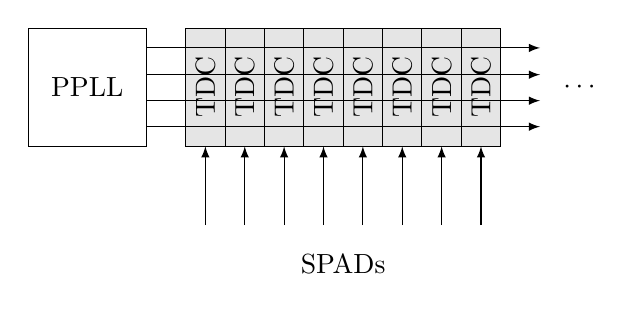
\begin{tikzpicture}

\draw  (-3.25,3) rectangle (-1.75,1.5) node[pos=.5]{PPLL};

\draw [fill=gray!20] (-1.25,3) rectangle (-0.75,1.5) node[pos=.5, rotate=90]{TDC};
\draw [fill=gray!20] (-0.75,3) rectangle (-0.25,1.5) node[pos=.5, rotate=90]{TDC};
\draw [fill=gray!20] (-0.25,3) rectangle (0.25,1.5) node[pos=.5, rotate=90]{TDC};
\draw [fill=gray!20] (0.25,3) rectangle (0.75,1.5) node[pos=.5, rotate=90]{TDC};
\draw [fill=gray!20] (0.75,3) rectangle (1.25,1.5) node[pos=.5, rotate=90]{TDC};
\draw [fill=gray!20] (1.25,3) rectangle (1.75,1.5) node[pos=.5, rotate=90]{TDC};
\draw [fill=gray!20] (1.75,3) rectangle (2.25,1.5) node[pos=.5, rotate=90]{TDC};
\draw [fill=gray!20] (2.25,3) rectangle (2.75,1.5) node[pos=.5, rotate=90]{TDC};

\draw [>=latex, ->] (-1.75,2.75) -- (3.25,2.75);
\draw [>=latex, ->] (-1.75,2.41) -- (3.25,2.41);
\draw [>=latex, ->] (-1.75,2.08) -- (3.25,2.08);
\draw [>=latex, ->] (-1.75,1.75) -- (3.25,1.75);

\draw [>=latex, ->] (-1,0.5) -- (-1,1.5);
\draw [>=latex, ->] (-0.5,0.5) -- (-0.5,1.5);
\draw [>=latex, ->] (0,0.5) -- (0,1.5);
\draw [>=latex, ->] (0.5,0.5) -- (0.5,1.5);
\draw [>=latex, ->] (1,0.5) -- (1,1.5);
\draw [>=latex, ->] (1.5,0.5) -- (1.5,1.5);
\draw [>=latex, ->] (2,0.5) -- (2,1.5);
\draw [>=latex, ->] (2.5,0.5) -- (2.5,1.5);

\node at (3.75,2.25) {$\cdots$};
\node at (0.75,0) {SPADs};
\end{tikzpicture}
    \caption{TDC line connected to PLL}
    \label{tkz:TDC_line_PLL}
\end{figure}

\subsection{Histogram}
Depending on whether an energy threshold is used or not, the data must be stored in a histogram. If no energy threshold is needed, one can simply add all the timestamps together and divide by the amount of observed counts to get a simple  average. For more sophisticated signal processing however, more data needs to be transferred to the FPGA than just an average. One can either read every TDC value directly into the FPGA, but for the expected amount of traffic, this  is not feasible. Therefore a histogram is necessary to condense the data into a smaller package without losing essential information. Considering that a histogram will be needed for every SPAD, the amount of space on the chip that the histograms can turn out to be quite large. 

The amount of bits required per SPAD are dependent on the bin size, resolution and bandwidth, and can be calculated using \cref{eq:histogram_bits}. 

\begin{equation}
		\text{bits} = \text{SPADs}\cdot\lceil \log_2(\text{binsize}) \rceil\cdot \lceil \frac{\text{bandwidth}}{\text{resolution}}\rceil
		\label{eq:histogram_bits}
\end{equation}

The next step is to investigate the limitations of these variables. First of all, the resolution is very important for both the accuracy of the device and the performance of the energy detection. The latter has a direct relationship with the power of the laser. Lowering the resolution will effectively decrease the peak power of the signal, because the power is effectively distributed over the length of a single bin. It is assumed that the FWHM of the laser is $100\,ps$i. So in order to ensure that at least one bin is exposed to the signal pulse in it's entire duration, one needs a resolution of $50\,ps$. This is also the resolution that is considered for the TDC. The bin size is dependent on the light intensity, which will increase when approaching Europa. The bandwidth allows for some flexibility. For example, when the previous measurements where close to 8 km the device can't travel far from that altitude in the next second. The next measurement will most likely also not yield an altitude further away than the previous one. Therefore the bandwidth can be limited to some extend, and adjusted between measurements.

\subsection{On chip signal processing}
When a histogram is constructed one can decide to process the data on the chip before sending it to the FPGA. This limits the complexity of the processing step however. It is difficult to implement a reasonable dynamic threshold for every individual histogram, and more complex waveforms that utilize known characteristics of the signal and noise photons other than intensity becomes infeasible. However a simple circuit that only sends the largest peak, or eliminates all values before the threshold is possible. 

\subsection{connection to FPGA}
The information stored in the histograms needs to be transported to the FPGA. There are several approaches that can be used to do this. The first possibility is a simple serial shift register to transport the data to the FPGA. A schematic of this is shown in \cref{tkz:serial_no_shadow}. This is a relatively slow solution, and the device cannot be used to receive photons during it, but this solution is very resource efficient.

\begin{figure}[H]
    \centering

\begin{tikzpicture}[scale=.5]


%% serial no shadowlatch
    \draw  (4,1) rectangle (6,-5);
    \draw (5,1) to (5,2) to (8,2)[>=latex,->]  to (8,1);
    \draw (2,-5) to (2,-6) to (5,-6)[>=latex,->] to (5,-5);
    \draw  (1,1) rectangle (3,-5);

    \draw  (10,1) rectangle (12,-5);
    \draw (11,1) to (11,2) to (13,2)[>=latex,->]  to (13,-2)  to (14,-2);
    \draw (8,-5) to (8,-6) to (11,-6)[>=latex,->] to (11,-5);
    \draw  (7,1) rectangle (9,-5);

    \draw  (14,0) rectangle (16,-4);

\end{tikzpicture}
    \caption{Method of transporting data from TDCs to the FPGA using a one bit serial shift register without shadowlatches}
    \label{tkz:serial_no_shadow}
\end{figure}


A second option is to include shadow latches in the design. A schematic is shown in \cref{tkz:serial_shadow}. This allows the device to continue operation during readout but one needs twice as much storage to achieve this.

\begin{figure}[H]
    \centering

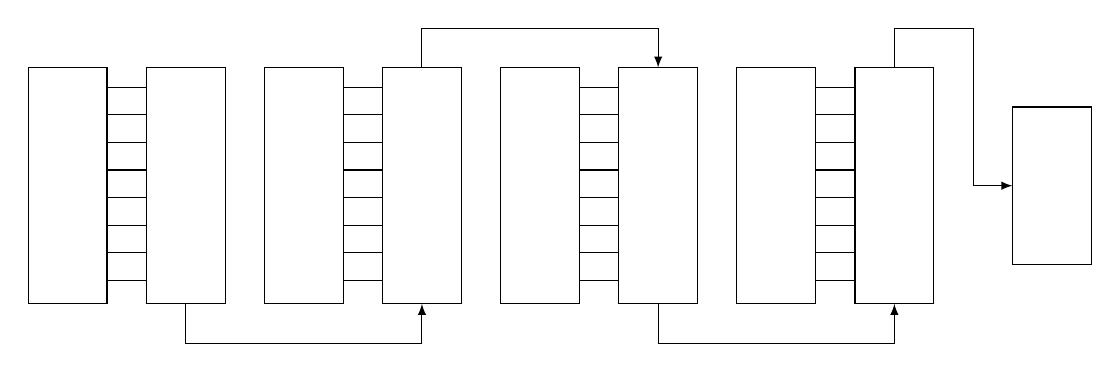
\begin{tikzpicture}[scale=.5]


%% serial shadowlatch
\draw  (28,1) rectangle (30,-5);
\draw (29,1) to (29,2) to (35,2)[>=latex,->]  to (35,1);
\draw (23,-5) to (23,-6) to (29,-6)[>=latex,->] to (29,-5);
\draw  (22,1) rectangle (24,-5);

\draw  (40,1) rectangle (42,-5);
\draw (41,1) to (41,2) to (43,2)[>=latex,->]  to (43,-2)  to (44,-2);
\draw (35,-5) to (35,-6) to (41,-6)[>=latex,->] to (41,-5);
\draw  (34,1) rectangle (36,-5);

\draw  (44,0) rectangle (46,-4);

\draw  (25,1) rectangle (27,-5);
\draw
(27,0.5)   to (28,0.5)
(27,-0.2) to (28,-0.2)
(27,-0.9)  to (28,-0.9)
(27,-1.6) to (28,-1.6)
(27,-2.3) to (28,-2.3)
(27,-3) to (28,-3)
(27,-3.7) to (28,-3.7)
(27,-4.4) to (28,-4.4);

\draw  (31,1) rectangle (33,-5);
\draw
(33,0.5)   to (34,0.5)
(33,-0.2) to (34,-0.2)
(33,-0.9)  to (34,-0.9)
(33,-1.6) to (34,-1.6)
(33,-2.3) to (34,-2.3)
(33,-3) to (34,-3)
(33,-3.7) to (34,-3.7)
(33,-4.4) to (34,-4.4);

\draw  (37,1) rectangle (39,-5);
\draw
(39,0.5)   to (40,0.5)
(39,-0.2) to (40,-0.2)
(39,-0.9)  to (40,-0.9)
(39,-1.6) to (40,-1.6)
(39,-2.3) to (40,-2.3)
(39,-3) to (40,-3)
(39,-3.7) to (40,-3.7)
(39,-4.4) to (40,-4.4);

\draw  (19,1) rectangle (21,-5);
\draw
(21,0.5)   to (22,0.5)
(21,-0.2) to (22,-0.2)
(21,-0.9)  to (22,-0.9)
(21,-1.6) to (22,-1.6)
(21,-2.3) to (22,-2.3)
(21,-3) to (22,-3)
(21,-3.7) to (22,-3.7)
(21,-4.4) to (22,-4.4);


\end{tikzpicture}
    \caption{Method of transporting data from TDCs to the FPGA using a one bit serial shift register without shadowlatches}
    \label{tkz:serial_no_shadow}
\end{figure}


A third option is to use the same shadow latches, but read them out in parallel. This can be done at a faster pace than the previous designs. A schematic is shown in \cref{tkz:parallel_shadow}. 

\begin{figure}[H]
    \centering

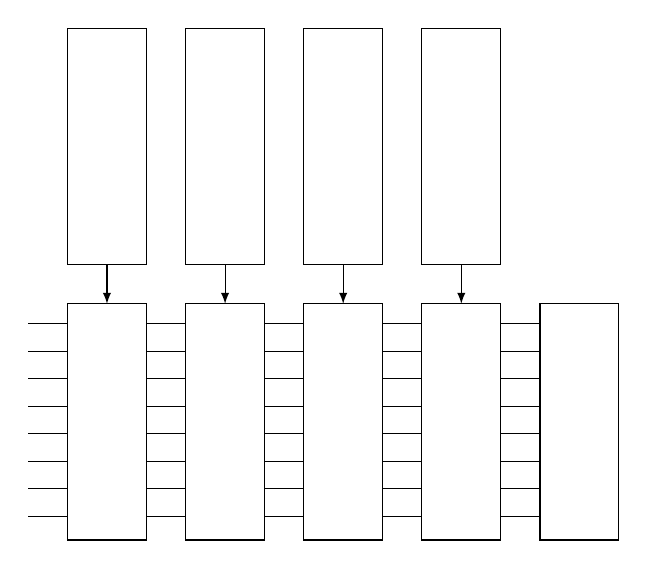
\begin{tikzpicture}[scale=.5]

\draw  (1,-15) rectangle (3,-21);
\draw
(3,-15.5)   to (4,-15.5)
(3,-16.2) to (4,-16.2)
(3,-16.9)  to (4,-16.9)
(3,-17.6) to (4,-17.6)
(3,-18.3) to (4,-18.3)
(3,-19) to (4,-19)
(3,-19.7) to (4,-19.7)
(3,-20.4) to (4,-20.4);

\draw  (4,-15) rectangle (6,-21);
\draw
(6,-15.5)   to (7,-15.5)
(6,-16.2) to (7,-16.2)
(6,-16.9)  to (7,-16.9)
(6,-17.6) to (7,-17.6)
(6,-18.3) to (7,-18.3)
(6,-19) to (7,-19)
(6,-19.7) to (7,-19.7)
(6,-20.4) to (7,-20.4);

\draw  (7,-15) rectangle (9,-21);
\draw
(9,-15.5)   to (10,-15.5)
(9,-16.2) to (10,-16.2)
(9,-16.9)  to (10,-16.9)
(9,-17.6) to (10,-17.6)
(9,-18.3) to (10,-18.3)
(9,-19) to (10,-19)
(9,-19.7) to (10,-19.7)
(9,-20.4) to (10,-20.4);

\draw  (10,-15) rectangle (12,-21);
\draw
(0,-15.5)   to (1,-15.5)
(0,-16.2) to (1,-16.2)
(0,-16.9)  to (1,-16.9)
(0,-17.6) to (1,-17.6)
(0,-18.3) to (1,-18.3)
(0,-19) to (1,-19)
(0,-19.7) to (1,-19.7)
(0,-20.4) to (1,-20.4);

\draw  (13,-15) rectangle (15,-21);
\draw
(12,-15.5)   to (13,-15.5)
(12,-16.2) to (13,-16.2)
(12,-16.9)  to (13,-16.9)
(12,-17.6) to (13,-17.6)
(12,-18.3) to (13,-18.3)
(12,-19) to (13,-19)
(12,-19.7) to (13,-19.7)
(12,-20.4) to (13,-20.4);

\draw  (1,-14) rectangle (3,-8);
\draw  (4,-14) rectangle (6,-8);
\draw  (7,-14) rectangle (9,-8);
\draw  (10,-14) rectangle (12,-8);

\draw [>=latex,->](2,-14) to (2,-15);
\draw [>=latex,->](5,-14) to (5,-15);
\draw [>=latex,->](8,-14) to (8,-15);
\draw [>=latex,->](11,-14) to (11,-15);

\end{tikzpicture}
    \caption{Method of transporting data from TDCs to the FPGA using a one bit serial shift register without shadowlatches}
    \label{tkz:serial_no_shadow}
\end{figure}


Considering the fact that one wants to measure for as short a time as possible, there is most likely enough time to transport the data at a small pace before the device needs to measure again. Therefore the investment into shadow latches is not worth it. A simple serial shift register would be the best fit in this case.



